%!TEX option = -shell-escape
% Document type
\documentclass[10pt, titlepage, a4paper]{article}



	% Packages


        \usepackage{graphicx}
	\usepackage{amsmath}
  \usepackage[utf8]{inputenc}
	\usepackage{amsfonts}
	\usepackage{fancyhdr}
	\usepackage{enumerate}
	\usepackage{listings}
    \usepackage{minted}
	\usepackage[titletoc]{appendix}
	\usepackage[pdfborder={0 0 0},colorlinks=true, urlcolor=blue, citecolor=red, bookmarks=false]{hyperref}
	\usepackage[margin=3cm]{geometry}
\usepackage[absolute]{textpos}
	\usepackage[section]{placeins}
	\usepackage{url}
	\usepackage{tabularx}
%	\usepackage{gensymb}
	\usepackage{caption}
  \usepackage{subcaption}
  \usepackage{float}
  \usepackage{mathtools}
  \usepackage{amssymb}
  \usepackage{algpseudocode}

%	\usepackage{xltxtra}
	% Page style
	\pagestyle{fancy}
	\marginparsep = 0pt
  \graphicspath{ {figures/} }



	% Set font
	%\setromanfont{Calibri}

	\renewcommand\contentsname{Contents}
	\newcommand{\HRule}{\rule{\linewidth}{0.5mm}}
	\renewcommand{\abstractname}{Abstract}


	\newcommand{\circR}{\textsuperscript{\textregistered}}

	% Code style
	\lstset{
		backgroundcolor=\color[rgb]{0.92,0.92,0.92},
		basicstyle=\footnotesize,
		showspaces=false,
		showstringspaces=false,
		showtabs=false,
		tabsize=2,
		captionpos=b,
		breaklines=false,
		keywordstyle=\color[rgb]{0,0,1},
		commentstyle=\color[rgb]{0.133,0.545,0.133}
	}

\begin{document}
\begin{titlepage}
% Title
%\title{

\begin{center}
		\begin{figure}[t]
				
\includegraphics[width=15mm, bb=0 0 100 100]{MDHlogga.png}
		\end{figure}
                 	\Large M\"{a}lardalen University \\
			\Large School of Innovation Design and Engineering \\
                        \Large V\"{a}ster\r{a}s, Sweden\\

                        \noindent\makebox[\linewidth]{\rule{\textwidth}{0.4pt}}\\[0.5cm]

                %The complete name of the course you are enrolled in
                \Large{Bachelor Thesis}\\[2.0cm]

			\huge \textbf{\uppercase{Evolutionary computation in continuous optimization and machine learning}} \\ [2.5cm] %TITLE!!!!!!!!

			\LARGE Leslie Dahlberg \\
        	\large ldg14001@student.mdh.se \\[2.5cm]

\begin{flushleft}
			\Large Examiner: Peter Funk\\[0.5cm]
			\Large M\"{a}lardalen University\\
			\Large V\"{a}ster\r{a}s, Sweden\\[1.0cm]

			\Large Supervisor: Ning Xiong\\[0.5cm]
			\Large M\"{a}lardalen University\\
			\Large V\"{a}ster\r{a}s, Sweden\\[0.5cm]

\end{flushleft}

              \vspace*{\fill}
                    \large \today		%today should be replaced by the date the report is sent for examination

\end{center}

\end{titlepage}
%\date{}
%\maketitle

% Page style
\thispagestyle{fancy}
\fancyhead[R]{Leslie Dahlberg}
\fancyhead[L]{M\"{a}lardalen University}
\fancyfoot[L]{}
%\fancyfoot[LE,RO]{\thepage}
\renewcommand{\headrulewidth}{0.4pt}
\renewcommand{\footrulewidth}{0.4pt}

% Begin actual text

\def\abstract{
   \vfil
\begin{center}%
{\bfseries\abstractname\vspace{-.5em}}
\end{center}
\itshape
}

\def\endabstract{\par
}


\newpage


% ============================= Abstract ==============================
\begin{abstract}
{\color{blue} Det h\"ar avsnittet ska helt enkelt vara just detta: en sammanfattning av hela rapporten. En l\"amplig omfattning \"ar c:a 200 - 250 ord.  En bra tumregel \"ar att sammanfattningen ska h\r{a}llas s\r{a} kort det g\r{a}r, den ska vara kompakt men fortfarande tydlig, informativ och v\"acka intresse. Ge de viktigaste fakta och summera allt det som \"ar v\"asentligt i rapporten.  F\"oljande b\"or ing\r{a}:
\begin{itemize}
\item Presentation/introduktion av omr\r{a}det f\"or arbetet,
\item \"Oversiktlig presentation av uppgiften inklusive syfte och fr\r{a}gest\"allning,
\item Motivation till varf\"or omr\r{a}det och uppgiften \"ar viktiga och intressanta,
\item Generell beskrivning av hur du angripit uppgiften, vad du har gjort,
\item Sammanfattning av resultat och slutsatser och vad ditt arbete bidrar med.
\end{itemize}

Inga detaljer ska vara med i sammanfattningen, inte heller beskrivning av hur rapporten \"ar uppst\"alld.

Sammanfattningen ska kunna l\"asas helt frist\r{a}ende fr\r{a}n resten av rapporten, och av en ganska bred grupp av l\"asare. Den ska ge en bra grund f\"or att en l\"asare ska kunna bed\"oma om hen \"ar intresserad av att l\"asa hela rapporten.

Sammanfattningen \"ar den del av en rapport som l\"ases allra mest och av flest personer. D\"arf\"or \"ar det extra viktigt att du skriver en bra sammanfattning. Du beh\"over ha ett ordentligt grepp om inneh\r{a}llet i rapporten n\"ar du skriver sammanfattningen, och n\"ar hela rapporten \"ar klar b\"or du granska och vid behov revidera sammanfattningen s\r{a} att den \"overensst\"ammer med rapporten.}

\end{abstract}
\newpage
% ========================== Document version ===========================
%\begin{center}
%	\begin{tabular}{|l|l|l|}
 %
	%	\multicolumn{3}{c}{\textbf{{\large Document version}}} \\
	%	\hline
 	%	Version & Date & Note \\ \hline
 	%	 &  &  \\ \hline
	%	 &  &  \\ \hline
	%	 &  &  \\ \hline
	%	 &  &   \\ \hline
	%	 &  &   \\ \hline
	%	 &  &   \\ \hline
%	\end{tabular}
%\end{center}
%\newpage
%========================== Table of contents ===========================
\hypersetup{linkcolor=black}
\tableofcontents
\hypersetup{linkcolor=red}

\newpage

% ============================== Intro ===============================

\input{./introduction}

\input{./background}

\section{Related Work}

Ideas around evolutionary computation began emerging in 1950s. Several researchers, independently from each-other, created algorithms which were inspired by natural Darwinian principles, these include Holland's Genetic Algorithms, Schwefel's and Rechenberg's Evolution Strategies and Fogel's Evolutionary Programming. These pioneering algorithms shared the concepts of populations, individuals, offspring and fitness and ,compared to natural systems, they were quite simplistic, lacking gender, maturation processees, migration, etc~\cite{dejong2009EC}.

Research has shown that no single algorithm can perform better than all other algorithms on average. This has been referred to as the `no-free-lunch' and current solutions instead aim at finding better solutions to specific problems by exploiting inherent biases in the problem. This has led to the desire to classify different algorithms in order to decide which algorithms should be used in which situations, a problem which is not trivial~\cite{dejong2009EC}.

\subsection{Recent Research}

Recent research has focused, among others, on parallelism, multi-population models, multi-objective optimization, dynamic environments and evolving executable code. Parallelism can easily be exploited in EC because of it's inherently parallel nature, e.g each individual in a population can be evaluated, mutated and crossed-over independently. Multi-core CPUs, massively parallel GPUs, clusters and networks can be used to achieve this. Multi-population models mimic the way species depend on each other in nature. Examples of this include host-parasite and predator-prey relationships where the the individual's fitness is connected to the fitness of another individual. Multi-objective optimization aims to solve problems where conflicting interests exist, a good example would be optimizing for power and fuel-consumption simultaneously. In such problems the optimization algorithm has to keep two or more interests in mind simultaneously and find intersections points which offer the best trade-offs between them. Dynamic environments include things like the stock markets and traffic systems. Traditional EAs perform badly in these situations but they can perform well when slightly modified to fit the task. Evolving executable code, as in Genetic Programming and Evolutionary Programming, is a hard problem with very interesting potential applications. Most often low-level code such as assembly, lisp or generic rules are evolved~\cite{dejong2009EC}.

\subsection{Emerging Evolutionary Algorithms}

\paragraph{Differential Evolution}

Differential evolution (DE) was conceived in 1995 by Storn and Price~\cite{storn1995differential} and soon gained wide acceptance as one of the best algorithms in continuous optimization~\cite{price1997differential}. This spawned many new papers descibing variations and hybrids of the algorithm~\cite{5601760}, such as self-adaptive DE (SaDE)~\cite{qin2009differential}, opposition-based DE (ODE)~\cite{rahnamayan2008opposition} and DE with global and local neighborhoods (DEGL)~\cite{rahnamayan2008opposition}.

DE is very easy to implement and has been shown to outperform most other algorithms consistently, it has also been shown that it in general performs better than PSO~\cite{das2009differential, vesterstrom2004comparative}. DE uses very few patameters and the effects of altering these parameters have been well studied~\cite{5601760}. DE comes in a total of 10 different varieties based on which mutation and cross-over operators are used~\cite{price2006differential}. Eight of these schemes have been tested and compared, showing that the version called DE/best/1/bin (which utilizes the best current individual in the cross-over process instead of random invidivuals) generally yields the best results~\cite{mezura2006comparative}.~\cite{gamperle2002parameter} measured the performance of different combinations of parameters, producing general recommendations for DE.

The desire to find optimal parameters have led to the use of self-adjusting DE algorithms. Examples inlude the use of fuzzy systems to control the parameters~\cite{liu2005fuzzy} and the SaDE algorithm~\cite{qin2009differential}.

\paragraph{Particle Swarm Optimization}

Particle swarm optimization (PSO) is the most widely used swarm intelligence (SI) algorithm to date. Many modified versions of PSO have been proposed, among others quantum-behaved PSO (QPSO), bare-bones PSO (BBPSO), chaotic PSO, fuzzy PSO, PSOT-VAC and opposition-based PSO. PSO has also been hybridized with other evolutionary algorithm, for instance: genetic algorithms (GA), artificial immune systems (AIS), tabu search (TS), ant colony optimization (ACO), simulated annealing (SA), differential evolution (DE), bio-geography based optimization (BBO) and harmonic search (HS)~\cite{zhang2015comprehensive}.

Wang et al.~\cite{dang2012selection} have compared the performance of different PSO-parameters and proposed a set of criteria for improving the performance of PSO. Fuzzy logic controllers (FLC) have been used to continuously optimize the PSO-parameters by Kumar and Chaturvedi~\cite{kumar2011tuning}. Zhang et al. found a simple way to use control theory in order to find good parameters~\cite{zhang2011simple}. Yang proposed modified velocity PSO (MVPSO) in which particles learn the best parameters from the other particles~\cite{yang2011particle}.


\paragraph{Estimation of Distribution Algorithms}

Estimation of distribution algorithms (EDA) use probabilitic models to solve complex optimization problems. They have been successfull at many engineering problems which at which other algorithms have failed, for instance: millitary antenna design, protein structure prediction, clustering of genes, chemotherapy optimization, portfolio management, etc~\cite{Hauschild2011111}.

Several techniques have been proposed to make EDA more efficient. Parallelization of fitness evaluation and model building has proven effective~\cite{sastry2007towards}. Local optimization techniques such as deterministic hill climbing (DHC) has been shown to make EDA faster~\cite{hart1994adaptive}.

\subsection{Evolutionary Algorithms and Machine Learning}

Evolutionary algorithms (EC) and machine learning (ML) are two growing and promising field in computer science and many attempts have therefore been made to combine the two. ML has been used to improve EC optimization algorithms with so called MLEC-algorithms where various techniques from AI and ML, such as artificial neural networks (ANN), cluster analysis (CA), support vector machines (SVM), etc. help EC algorithms to learn important features of the search space~\cite{6052374}.

The opposite use case has also been proposed, using EC to improve ML techniques. An example of this is using DE to optimize feed-forward neural networks (FFNN). Here DE seems to perform similarly to traditional gradient based techniques~\cite{ilonen2003differential}. Hajare and Bawane showed that using PSO to initialize weights and biases in a neural network before training yields better results than using random weights and help avoid local minima which backpropagation (BP) algorithms often get stuck in~\cite{hajare2015feed}. Larra{\~n}aga and Lozano~\cite{larranaga2001estimation} tested various EC algorithms (GA, EDA and ES) agains BP and concluded that EC is a competetive alternative to traditional approaches.

\subsection{Contributions}

EC is a an interesting alternative to traditional approaches in machine learning and continuous optimization and while algorithms such as DE, PSO, etc. have been compared on mathematical benchmarks before~\cite{vesterstrom2004comparative, price1997differential}, the application of EC to machine learning has not been studied with as much details. My primary contribution to the field will be to find what algorithms work best for different ML problems och based on this propose ML-specific improvements.


\section{Problem Formulation}

The purpose of this thesis is to explore the performance and usefulness of three emerging evolutionary algorithms: differential evolution (DE), particle swarm optimization (PSO) and estimation of distribution algorithms (EDA). The intention is to compare these against each other on a set of benchmark functions and practical problems in machine learning and then, if possible, develop a new or modified algorithm which improves upon then aforementioned ones in some aspect.

\paragraph{Research Questions}

The questions asked in the thesis are:
\begin{itemize}
  \item How do DE, PSO and EDA perform comparatively when applied to mathematical optimization problems?
  \item How do DE, PSO and EDA perform comparatively when applied to machine learning problems such as neural network optimization and artificial intelligence in games
  \item How are DE, PSO and EDA suited to these different problems?
  \item Can an improved algorithm which draws inspiration from the design of DE, PSO and/or EDA outperform any of them in some/all of the aformentioned benchmarks and problem sets?
\end{itemize}

\paragraph{Motivation}

This research is interesting because it yield insight into the applicability of emerging evolutionary algorithms to currently popular machine learning methods such as artifical neural networks and also compares them more generally on generic mathematical optimization problems. The possibility of an improved novel algorithm which is better att handling machine learning problems also makes the work more interesting.

\paragraph{Outcomes}

The goals in this works are:
\begin{itemize}
  \item Benchmark DE, PSO, EDA on mathematical optimization problems
  \item Benchmark DE, PSO, EDA on machine learning problems
  \item Develop a new algorithm inspired by DE, PSO and/or EDA
  \item Benchmark the new algorithm
  \item Compare the new algorithm with DE, PSO and EDA and draw conclusions from the results
\end{itemize}

\paragraph{Limitations}

The scope of this work limits the number of algorithms which can be included in the testing. The individual algorithms also have numerous variations and parameters which can dramatically affect their behavior and it will not be possible to take all these considerations into account. Furthermore, the benchmarking will be restricted to a standard set of testing functions which may or may not provide reliable information regarding the general usability the algorithms. Since evolutionary algorithms have a large number of potential and actual use cases the practical testing will only concern a small subset of the these and may therefore not provide accurate data for all possible use cases.


\input{./method}

\section{Ethical and Societal Considerations}

This work does not have any ethical or societal considerations.


% =========================== Actual Content ==========================

\section{Experimental Results and Evaluation} \label{section:benchmark}

This section describes the design of five benchmarks ($F_{1-10}$, $FA_{1-6}$, $CLS_{1-7}$, $CLU_{1}$, $IGC_{1}$), presents the results of the measurements and discusses their significance.

%\section{Benchmark} \label{section:benchmark}

%This section describes all benchmark components and how they will be evaluated. The benchmark consists of a mathematical function optimization component and machine learning component.

\subsection{Mathematical Function Optimization ($F_{1-10}$)}

The functions $F_{1-10}$ for the mathematical function optimization benchmark have been taken from the 2005 CEC conference on continuous evolutionary optimization algorithms~\cite{suganthan2005problem}. Many functions from the well known DeJong test-bed are included~\cite{Whitley1996245}.

For all functions $x=[x_1,x_2,x_3,...,x_D]$ are the input parameters, $o=[o_1,o_2,o_3,...,o_D]$ is the global optimum, $D$ is the dimension and $M$ is an orthogonal matrix with parameters unique to each function. The matrices for $o$ and $M$ can be obtained from~\cite{suganthan2005problem}.
The functions are illustrated in two dimensions in figures~\ref{f1},~\ref{f2},~\ref{f3},~\ref{f4},~\ref{f5},~\ref{f6},~\ref{f7},~\ref{f8},~\ref{f9} and~\ref{f10}. The benchmark parameters and settings are listed in table~\ref{table:f1-10_params}.

\begin{table}[H]
  \centering
  \begin{center}
    \footnotesize
    \begin{tabular}{ | c | c | c | c | }
      \hline
      Parameter & Value (D=10) & Value (D=30) & Value (D=50) \\ \hline
      Repeat measurements & 30 & 30 & 30 \\ \hline
      Generations & 667 & 1200 & 1429 \\ \hline
      Population Size & 150 & 250 & 350 \\ \hline
    \end{tabular}
  \end{center}
  \caption{Benchmark parameters for $F_{1-10}$}
  \label{table:f1-10_params}
\end{table}

\paragraph{Shifted Sphere Function ($F_1$)} Unimodal, Separable

\begin{minipage}{.5\textwidth}
  \[
    F_1(x)=\sum_{i=1}^{D}{z_i^2}
  \]
  \[ z=x-o \]
  \[ x \in [-100,100]^D \]
\end{minipage}%
\begin{minipage}{.5\textwidth}
  \begin{figure}[H]
    \centering
    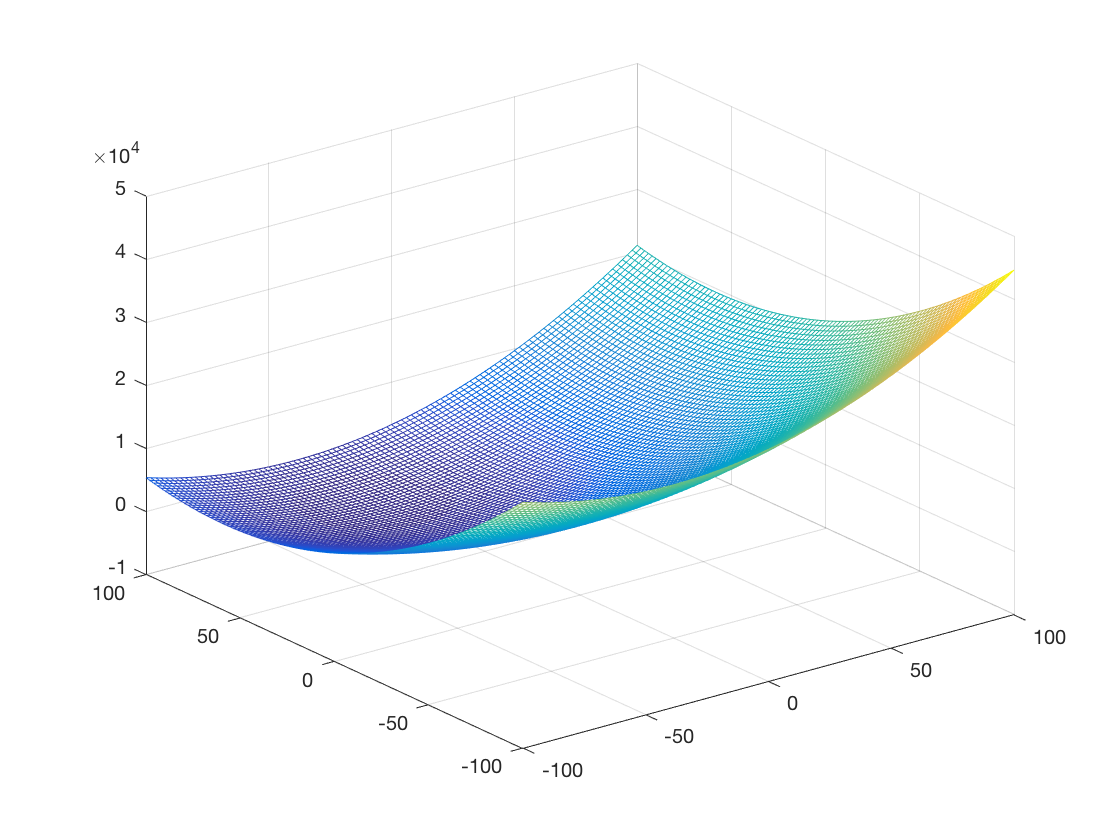
\includegraphics[width=0.7\linewidth]{f1}
    \caption{3-D map for 2-D function}
    \label{f1}
  \end{figure}
\end{minipage}


\paragraph{Shifted Schwefel’s Problem ($F_2$)} Unimodal, Non-Separable

\begin{minipage}{.5\textwidth}
\[
  F_2(x)=\sum_{i=1}^{D}{(\sum_{j=1}^{i}{z_j})^2}
\]
\[ z=x-o \]
\[ x \in [-100,100]^D \]
\end{minipage}%
\begin{minipage}{.5\textwidth}
  \begin{figure}[H]
    \centering
    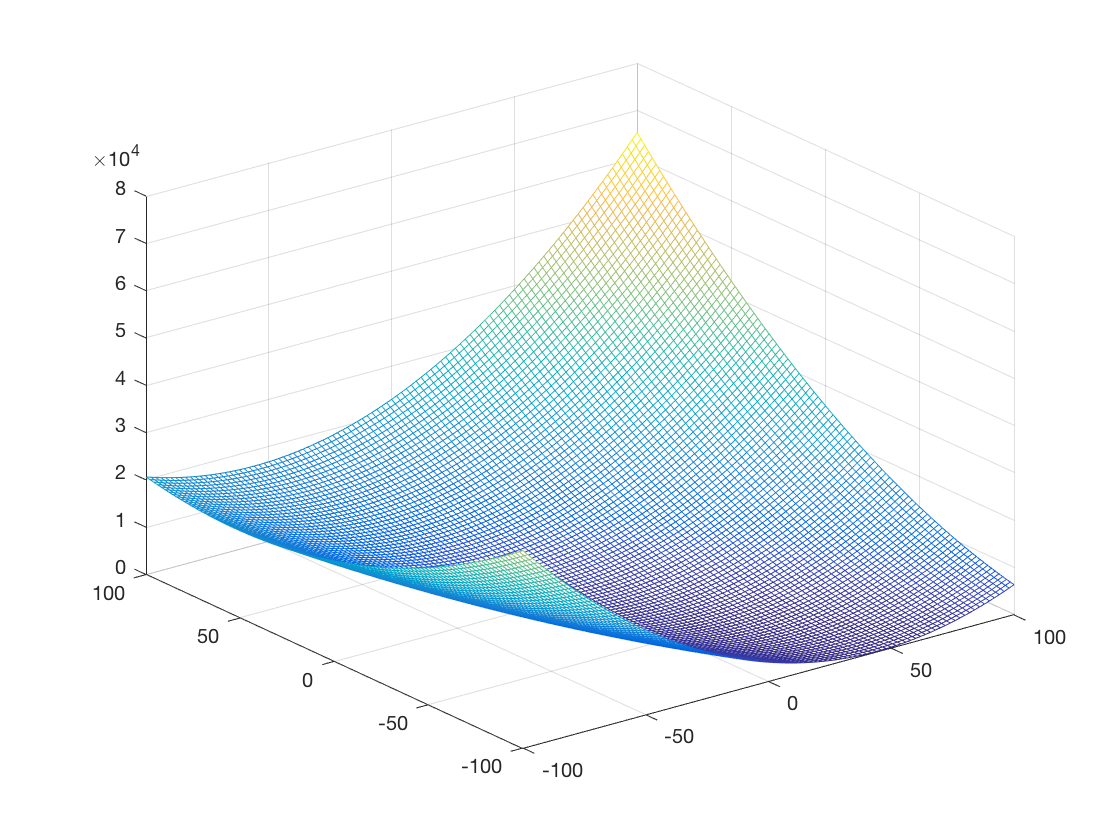
\includegraphics[width=0.7\linewidth]{f2}
    \caption{3-D map for 2-D function}
    \label{f2}
  \end{figure}
\end{minipage}


\paragraph{Shifted Rotated High Conditioned Elliptic Function ($F_3$)} Unimodal, Non-Separable

\begin{minipage}{.5\textwidth}
\[
  F_3(x)=\sum_{i=1}^{D}{(10^6)^{\frac{i-1}{D-1}}z_i^2}
\]
\[ z=(x-o)*M \]
\[ x \in [-100,100]^D \]
\end{minipage}%
\begin{minipage}{.5\textwidth}
  \begin{figure}[H]
    \centering
    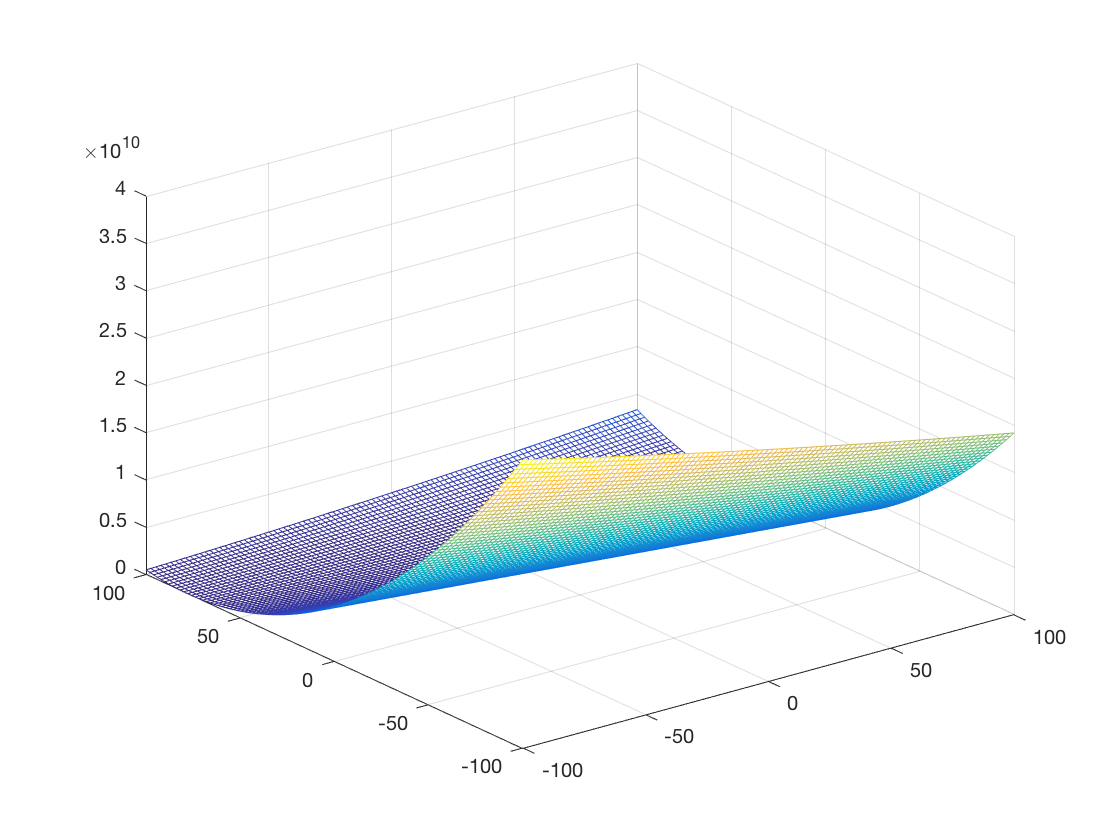
\includegraphics[width=0.7\linewidth]{f3}
    \caption{3-D map for 2-D function}
    \label{f3}
  \end{figure}
\end{minipage}


\paragraph{Shifted Schwefel’s Problem with Noise in Fitness ($F_4$)} Unimodal, Non-Separable

\begin{minipage}{.5\textwidth}
\[
  F_4(x)=(\sum_{i=1}^{D}{(\sum_{j=1}^{i}{z_j})^2})*(1+0.4|N(0,1)|)
\]
\[ z=x-o \]
\[ x \in [-100,100]^D \]
\end{minipage}%
\begin{minipage}{.5\textwidth}
  \begin{figure}[H]
    \centering
    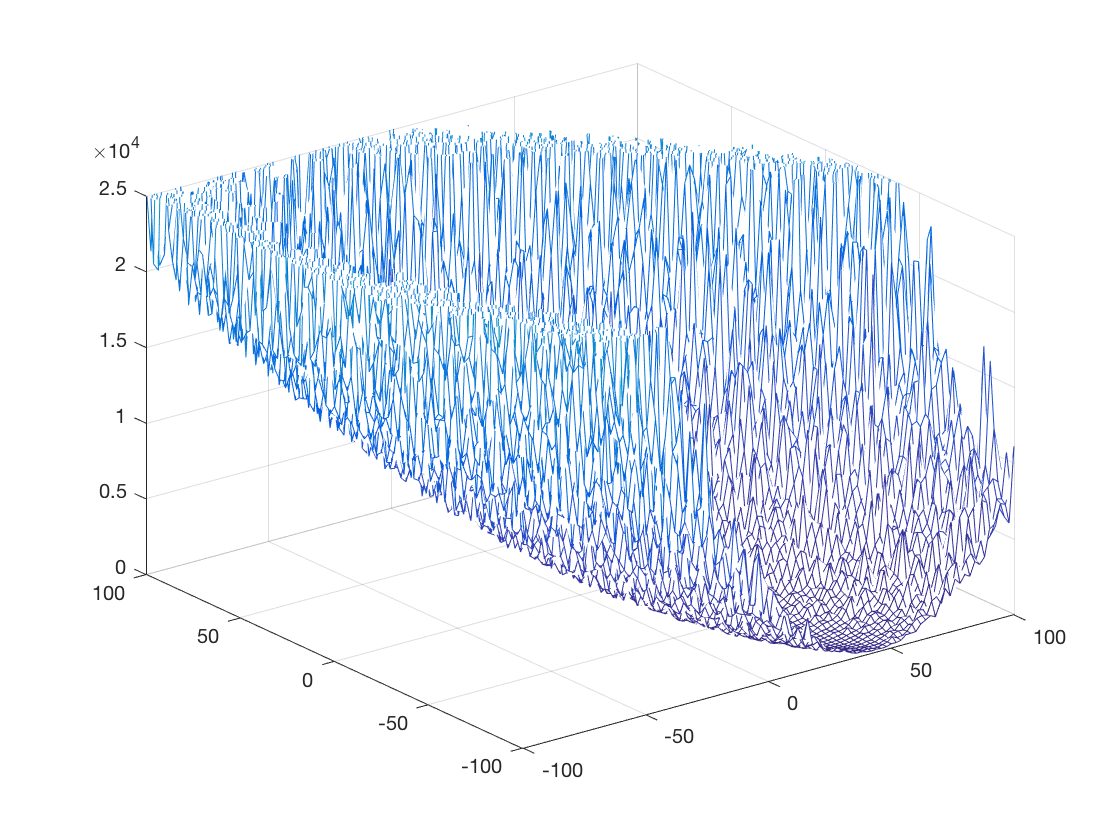
\includegraphics[width=0.7\linewidth]{f4}
    \caption{3-D map for 2-D function}
    \label{f4}
  \end{figure}
\end{minipage}


\paragraph{Schwefel’s Problem with Global Optimum on Bounds ($F_5$)} Unimodal, Non-Separable

\begin{minipage}{.5\textwidth}
\[
  F_5(x)=max\{|A_ix-B_i|\}
\]
\[ i=1,...,D, x \in [-100,100]^D \]
\[ A \text{ is a } D*D \text{ matrix}, a_{ij} = \text{ random numbers in } [-500,500],  det(A) \neq 0 \]
\[ B_i = A_i * o, o_i = \text{ random numbers in } [-100,100] \]
\[ o_i = -100 \text{, for } i=1,2,...,[D/4], o_i = 100 \text{, for } i=[3D/4],...,D \]
\end{minipage}%
\begin{minipage}{.5\textwidth}
  \begin{figure}[H]
    \centering
    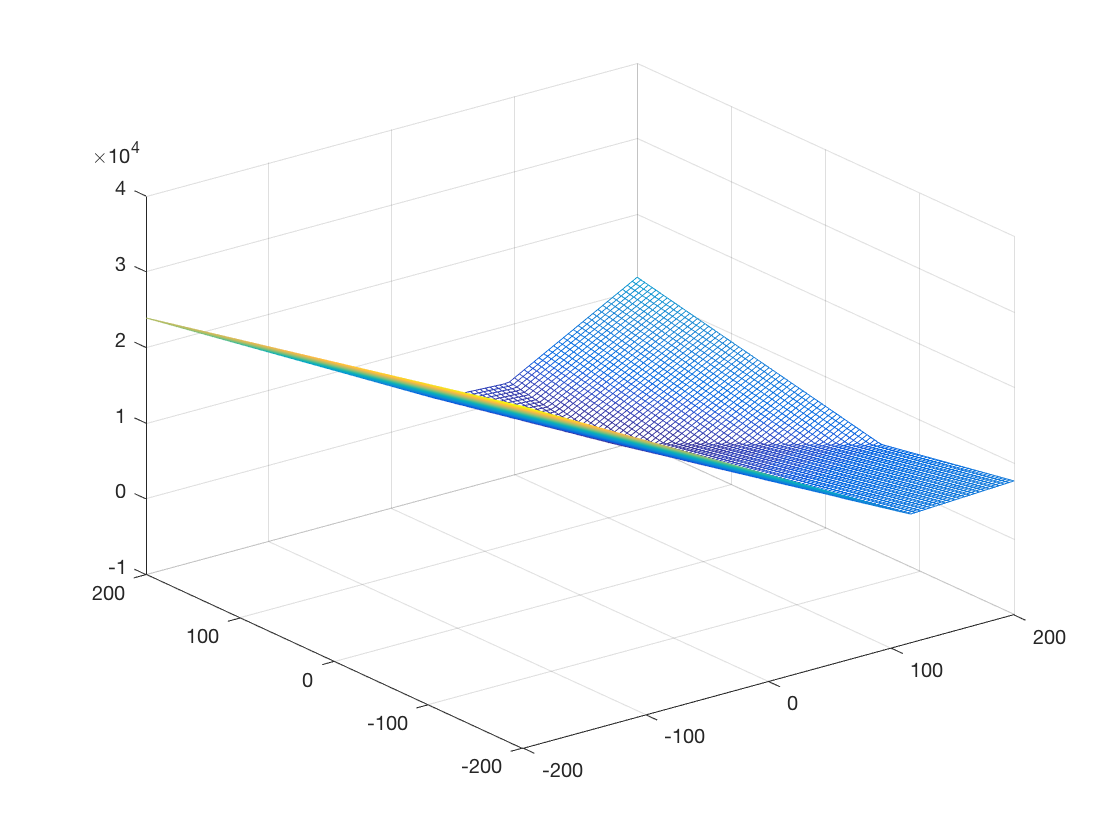
\includegraphics[width=0.7\linewidth]{f5}
    \caption{3-D map for 2-D function}
    \label{f5}
  \end{figure}
\end{minipage}


\paragraph{Shifted Rosenbrock’s Function ($F_6$)} Multimodal, Non-Separable

\begin{minipage}{.5\textwidth}
\[
  F_6(x)=\sum_{i=1}^{D-1}{(100(z_i^2 - z_{i+1})^2 + (z_i - 1)^2)}
\]
\[ z=x-o+1 \]
\[ x \in [-100,100]^D \]
\end{minipage}%
\begin{minipage}{.5\textwidth}
  \begin{figure}[H]
    \centering
    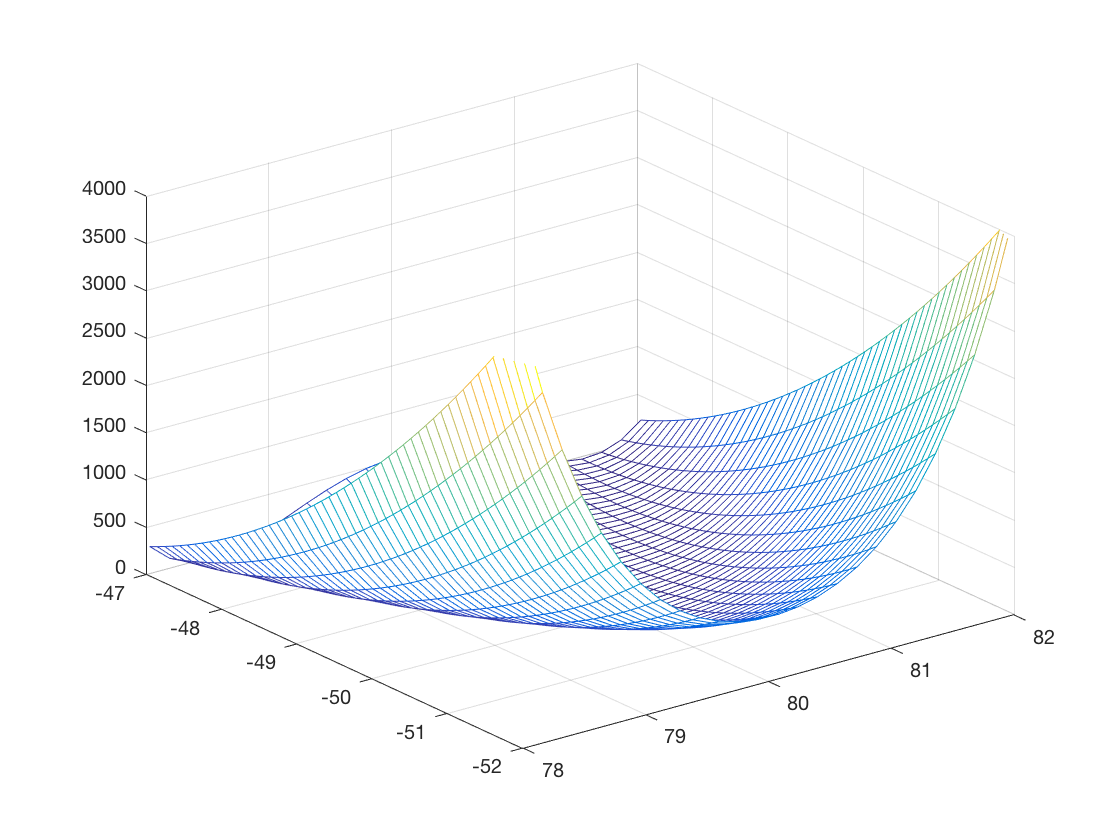
\includegraphics[width=0.7\linewidth]{f6}
    \caption{3-D map for 2-D function}
    \label{f6}
  \end{figure}
\end{minipage}


\paragraph{Shifted Rotated Griewank’s Function without Bounds ($F_7$)} Multimodal, Non-Separable

\begin{minipage}{.5\textwidth}
\[
  F_7(x)=\sum_{i=1}^{D}{\frac{z_i^2}{4000}}-\prod_{i=1}^{D}{\cos{\frac{z_i}{\sqrt{i}}}}+1
\]
\[ z=(x-o)*M \]
\[ x \in [0,600]^D \]
\end{minipage}%
\begin{minipage}{.5\textwidth}
  \begin{figure}[H]
    \centering
    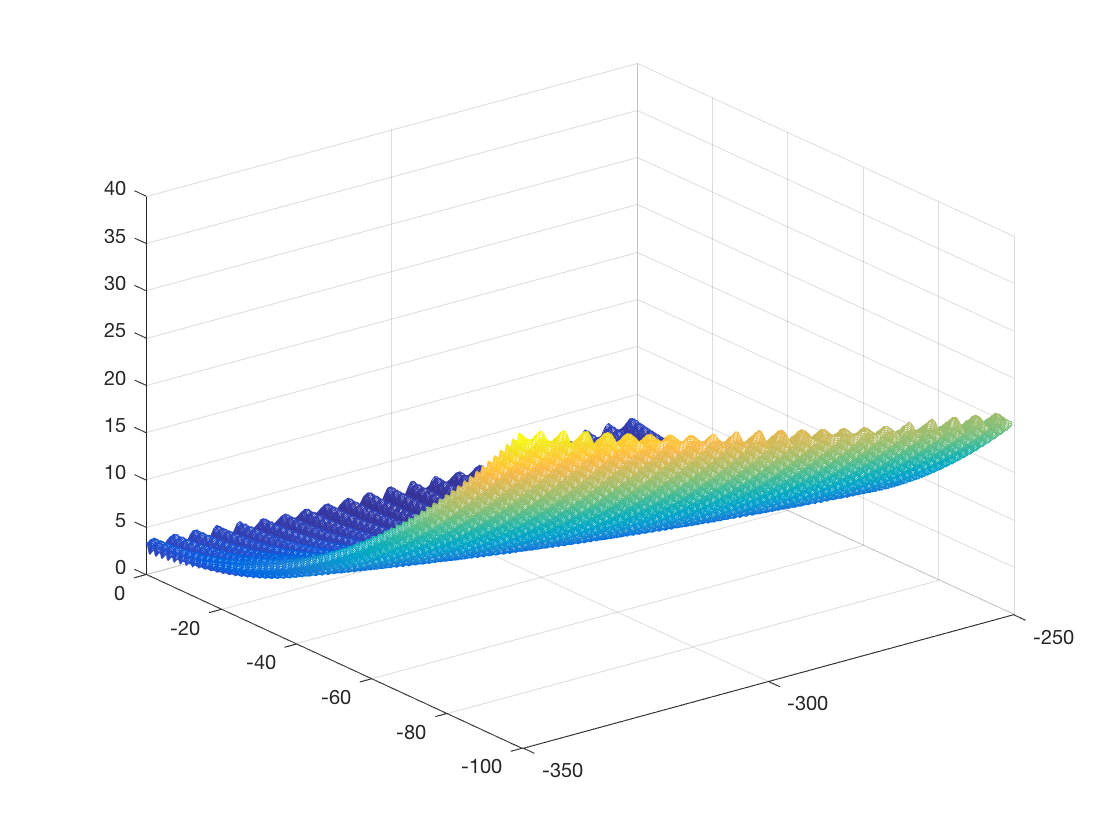
\includegraphics[width=0.7\linewidth]{f7}
    \caption{3-D map for 2-D function}
    \label{f7}
  \end{figure}
\end{minipage}

\paragraph{Shifted Rotated Ackley’s Function with Global Optimum on Bounds ($F_8$)} Multimodal, Non-Separable

\begin{minipage}{.5\textwidth}
\[
  F_8(x)=-20\exp{(-0.2\sqrt{\frac{1}{D}\sum_{i=1}^{D}{z_i^2}})}-\exp{(\frac{1}{D}\sum_{i=1}^{D}{\cos{(2\pi z_i)}})} + 20 + e
\]
\[ z=(x-o)*M \]
\[ x \in [-32,32]^D \]
\end{minipage}%
\begin{minipage}{.5\textwidth}
  \begin{figure}[H]
    \centering
    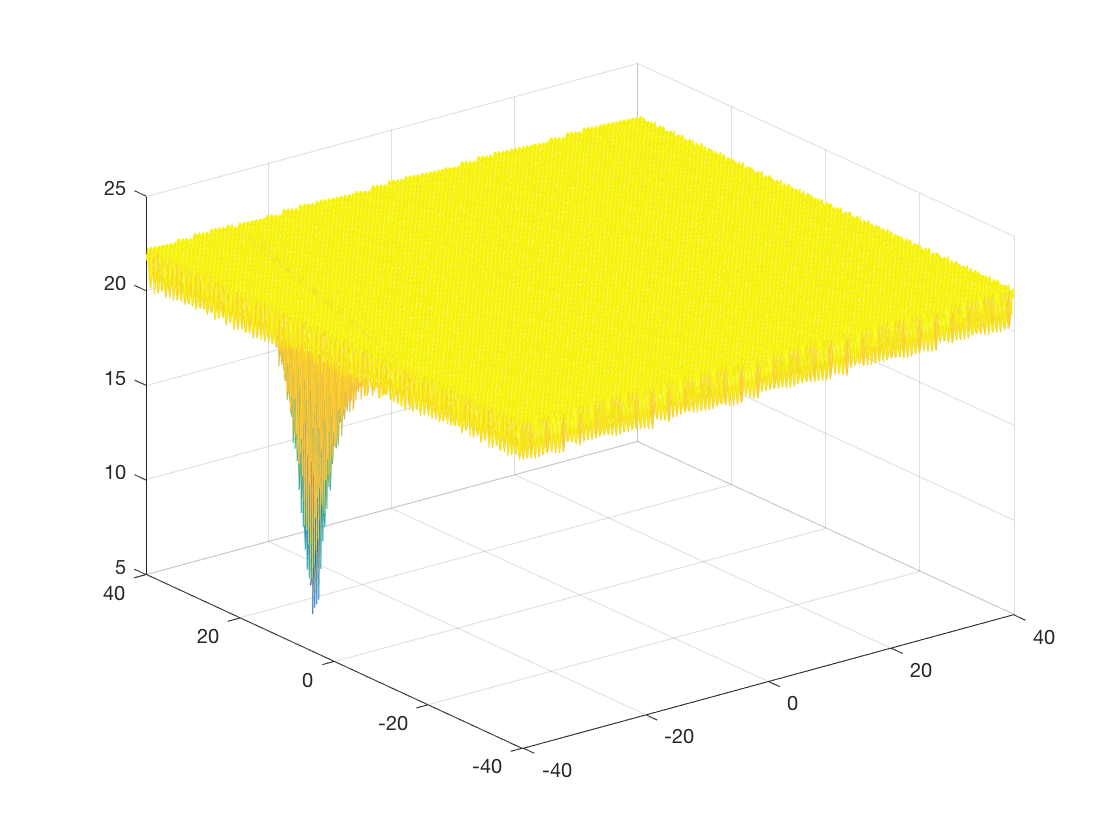
\includegraphics[width=0.7\linewidth]{f8}
    \caption{3-D map for 2-D function}
    \label{f8}
  \end{figure}
\end{minipage}

\paragraph{Shifted Rastrigin’s Function ($F_9$)} Multimodal, Separable

\begin{minipage}{.5\textwidth}
\[
  F_9(x)=\sum_{i=1}^{D}{z_i^2 - 10\cos{(2\pi z_i)} + 10}
\]
\[ z=x-o \]
\[ x \in [-5,5]^D \]
\end{minipage}%
\begin{minipage}{.5\textwidth}
  \begin{figure}[H]
    \centering
    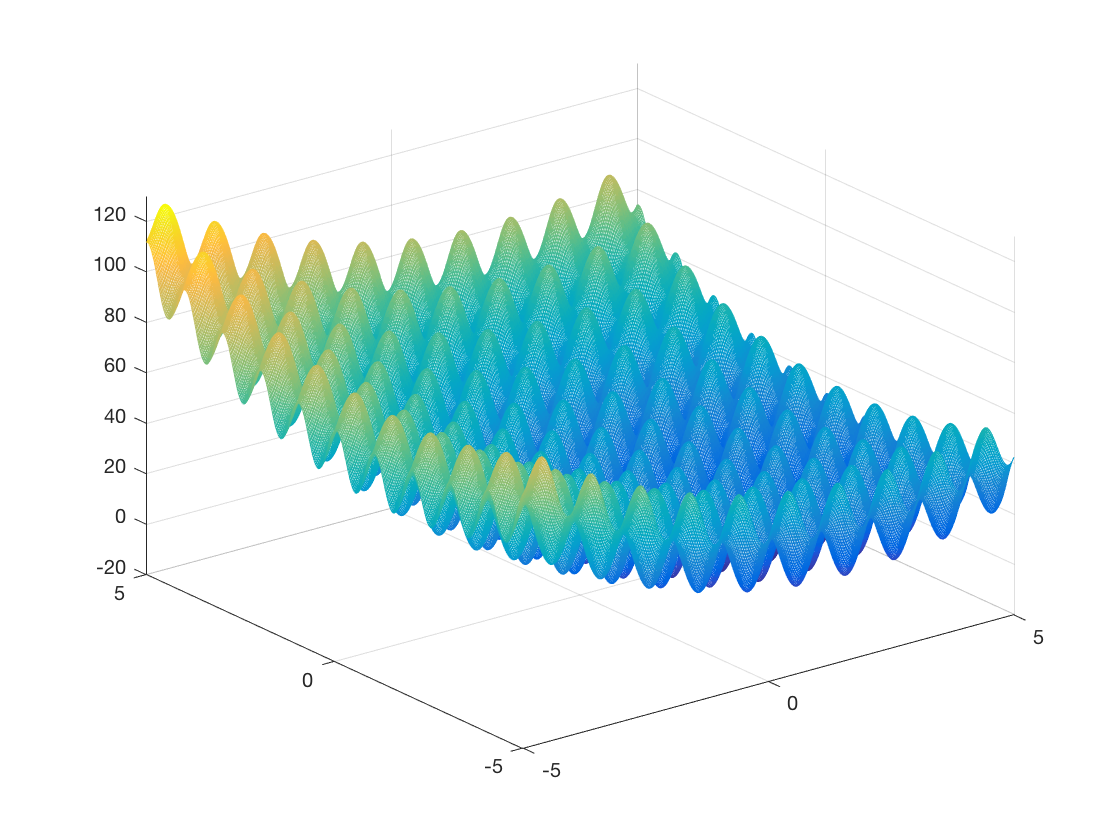
\includegraphics[width=0.7\linewidth]{f9}
    \caption{3-D map for 2-D function}
    \label{f9}
  \end{figure}
\end{minipage}


\paragraph{Shifted Rotated Rastrigin’s Function ($F_{10}$)} Multimodal, Non-Separable

\begin{minipage}{.5\textwidth}
\[
  F_{10}(x)=\sum_{i=1}^{D}{z_i^2 - 10\cos{(2\pi z_i)} + 10}
\]
\[ z=(x-o)*M \]
\[ x \in [-5,5]^D \]
\end{minipage}%
\begin{minipage}{.5\textwidth}
  \begin{figure}[H]
    \centering
    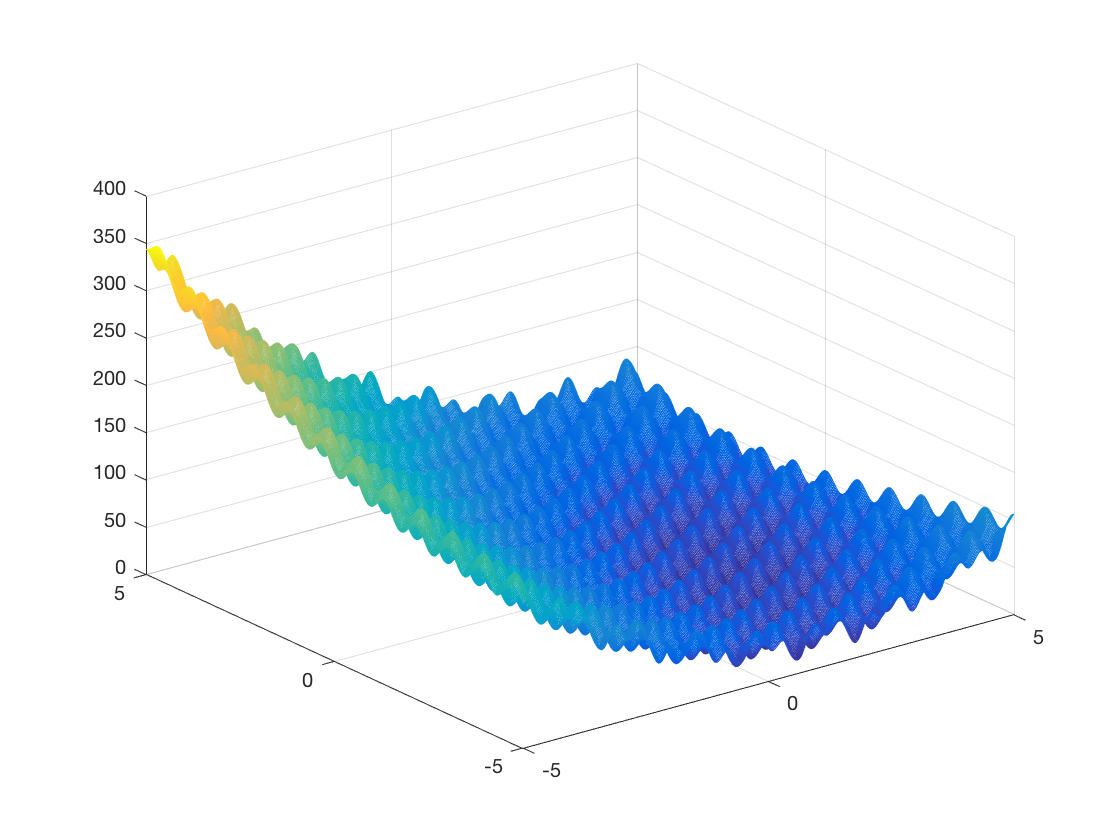
\includegraphics[width=0.7\linewidth]{f10}
    \caption{3-D map for 2-D function}
    \label{f10}
  \end{figure}
\end{minipage}

%\subsection{Machine Learning}

%This section describes the machine learning benchmarks, which primarily utilize feed-forward neural networks.

%To evaluate the optimization algorithms further I set have set out to apply them on a variety of machine learning problems. These will predominantly be applications of feed-forward neural networks (FFNN). The design of the neural network is one input layer with a size based on the problem dimension, two hidden layers and one output layer. I have chosen to use two hidden layers to make sure a good solution can be found quickly~\cite{329294}. The size of the hidden layers was set to $2/3$ and $1/3$ of the mean of the size of the input and output layers.

\subsection{Function Approximation ($FA_{1-6}$)}

The optimization algorithms were used find the optimal weights for feed-forward neural networks. The neural networks were evaluated on six function approximation data-sets which are available in Matlab's Neural Network Toolbox. The benchmark parameters and settings are listed in table~\ref{table:fa1-6_params}. The data-sets are listed in table~\ref{table:fa1-6_data-sets}.

\begin{table}[H]
  \centering
  \begin{center}
    \footnotesize
    \begin{tabular}{ | c | c | }
      \hline
      Parameter & Value \\ \hline
      Repeat measurements & 5 \\ \hline
      Generations & 250 \\ \hline
      Population Size & 50 \\ \hline
    \end{tabular}
  \end{center}
  \caption{Benchmark parameters for $FA_{1-6}$}
  \label{table:fa1-6_params}
\end{table}

\begin{table}[H]
  \centering
  \begin{center}
    \footnotesize
    \begin{tabular}{ | c | c | c | c | c | }
      \hline
      Data-set & Description & Input-Dimension & Output-Dimension & Weight-Dimension \\ \hline
      simplefit & Simple fitting & 1 & 1 & 4 \\ \hline
      bodyfat & Body fat percentage & 13 & 1 & 196 \\ \hline
      chemical & Chemical sensor & 8 & 1 & 81 \\ \hline
      cho & Cholesterol & 21 & 3 & 528 \\ \hline
      engine & Engine behavior  & 2 & 2 & 12 \\ \hline
      house & House value & 13 & 1 & 196 \\ \hline
    \end{tabular}
  \end{center}
  \caption{Data-sets for $FA_{1-6}$}
  \label{table:fa1-6_data-sets}
\end{table}

\paragraph{Evalutation Procedure}

The data sets contain two matrices. One with sample input vectors to the neural network and one with the expected correct output vectors. The function which the optimization algorithm directly optimizes is the sum of squared errors as defined by equation~\ref{eq:fa_fitness}

\begin{equation} \label{eq:fa_fitness}
  sse(x,t) = \frac{1}{2n} \sum_{i=1}^{n}{(y(x)-t)^2}
\end{equation}

where $x$ is the input vector to neural network $y$, $t$ is the correct expected output which $y(x)$ should produce and n is the length of vector $x$.

\subsection{Classification ($CLS_{1-7}$)}

The optimization algorithms were used find the optimal weights for feed-forward neural networks. The neural networks were evaluated on seven classification data-sets which are available in Matlab's Neural Network Toolbox. The benchmark parameters and settings are listed in table~\ref{table:cls1-7_params}. The data-sets are listed in table~\ref{table:cls1-7_data-sets}.

\begin{table}[H]
  \centering
  \begin{center}
    \footnotesize
    \begin{tabular}{ | c | c | }
      \hline
      Parameter & Value \\ \hline
      Repeat measurements & 5 \\ \hline
      Generations & 250 \\ \hline
      Population Size & 50 \\ \hline
    \end{tabular}
  \end{center}
  \caption{Benchmark parameters for $CLS_{1-7}$}
  \label{table:cls1-7_params}
\end{table}

\begin{table}[H]
  \centering
  \begin{center}
    \footnotesize
    \begin{tabular}{ | c | c | c | c | c | }
      \hline
      Data-set & Description & Input-Dimension & Output-Dimension & Weight-Dimension \\ \hline
      simpleclass & imple pattern recognition & 2 & 4 & 18 \\ \hline
      cancer & Breast cancer & 9 & 2 & 110 \\ \hline
      crab & Crab gender & 6 & 2 & 56 \\ \hline
      glass & Glass chemical & 9 & 2 & 110 \\ \hline
      iris & Iris flower & 4 & 3 & 35 \\ \hline
      thyroid & Thyroid function  & 21 & 3 & 528 \\ \hline
      wine & Italian wines & 13 & 3 & 224 \\ \hline
    \end{tabular}
  \end{center}
  \caption{Data-sets for $CLS_{1-7}$}
  \label{table:cls1-7_data-sets}
\end{table}


\paragraph{Evalutation Procedure}

Same as $FA_{1-6}$.

\subsection{Clustering ($CLU_{1}$)}

The optimization algorithms were used find the optimal weights for feed-forward neural networks. The neural networks were evaluated on one clustering data-set which is available in Matlab's Neural Network Toolbox. The benchmark parameters and settings are listed in table~\ref{table:clu1_params}. The data-sets are listed in table~\ref{table:clu1_data-sets}.

\begin{table}[H]
  \centering
  \begin{center}
    \footnotesize
    \begin{tabular}{ | c | c | }
      \hline
      Parameter & Value \\ \hline
      Repeat measurements & 5 \\ \hline
      Generations & 250 \\ \hline
      Population Size & 50 \\ \hline
    \end{tabular}
  \end{center}
  \caption{Benchmark parameters for $CLU_{1}$}
  \label{table:clu1_params}
\end{table}

\begin{table}[H]
  \centering
  \begin{center}
    \footnotesize
    \begin{tabular}{ | c | c | c | c | c | }
      \hline
      Data-set & Description & Input-Dimension & Output-Dimension & Weight-Dimension \\ \hline
      simplecluster & Simple clustering & 2 & 4 & 18 \\ \hline
    \end{tabular}
  \end{center}
  \caption{Data-sets for $CLU_{1}$}
  \label{table:clu1_data-sets}
\end{table}


\paragraph{Evalutation Procedure}

Same as $FA_{1-6}$.

\subsection{Intelligent Game Controllers ($IGC_{1}$)}


Machine learning test set $IGC_{1}$ uses evolutionary algorithms to evolve weights for feed-forward neural networks, which control the behavior of a game-agent in the classic game of ``Snake''. The benchmark parameters and settings are listed in table~\ref{table:fa1-6_params}.

\begin{table}[H]
  \centering
  \begin{center}
    \footnotesize
    \begin{tabular}{ | c | c | c | c | }
      \hline
      Parameter & Value  \\ \hline
      Individuals & 140 \\ \hline
      Generations & 1000 \\ \hline
      Grid dimension & 10*10 \\ \hline
      Weight dimension & 140 \\ \hline
      Repeat measurements & 10 \\ \hline
      Repeat fitness measurements & 5 \\ \hline
    \end{tabular}
  \end{center}
  \caption{Benchmark parameters for $FA_{1-6}$}
  \label{table:fa1-6_params}
\end{table}

\paragraph{Game Description and Rules}

The game is made up of a $n*m$ square grid through which a snake can freely move. The snake consists of a sequence of interconnected blocks and is divided into a head which moves in a certain direction and a tail which follows the head. Food blocks randomly appear on block at a time on the grid and the snake's objective is eat these blocks. When the snake's head touches the food block the block vanishes and the snake grows one square in length. If the head of the snake tries to move outside the grid it dies and the game ends. If the head of the snake collides with the tail it also and dies and the game ends. The snake's head can move in four direction: up, down, left and right. If the snake tries to move in the opposite of it's current direction it also dies. The snake has a starvation counter which forces it to pursue food and eat. The starvation counter is initialized to the starvation threshold when the game begins and decreases by one every time the snake moves. When the snake eats, the starvation counter is increased once by the starvation threshold. Figure~\ref{snake} illustrates the game grid. Figure~\ref{snake_alg} described the algorithm for the game. The game's parameters are explained in table~\ref{snake_p}.

\begin{figure}[H]
  \centering
  
\includegraphics[width=.3\linewidth]{snake}
  \caption{Snake $8*8$ game-field with snake hunting food}
  \label{snake}
\end{figure}


\begin{table}[H]
  \centering
  \begin{center}
    \begin{tabular}{ | c | c | }
      \hline
      Parameter & Description \\ \hline
      $D^2$ & Dimension of grid ($m*n$ blocks) \\ \hline
      $(x,y)$ & Starting point for snake head \\ \hline
      $d_s$ & Starting direction for snake head ($=\{left,right,up,down\}$) \\ \hline
      $t$ & Starvation threshold \\ \hline
    \end{tabular}
  \end{center}
  \caption{Parameters snake game}
  \label{snake_p}
\end{table}


\paragraph{Representation of Game State}

In order to control the snake with a neural network a representation of the state of the game has to be generated before each move. The chosen representation is a 12-dimensional vector in the range $[0,1]$. The initial default value of all dimensions is zero. Dimensions 1-4 indicates with a value of one whether any dangerous object (the tail or the edge of the grid) is immediately to the left, to the right, above or below the snake's head. Dimensions 5-8 indicate the distribution of the tail relative to the head of the snake. Floating-point numbers indicate how much of the tail is above, below, to the right and to the left of the head. Dimensions 9-12 indicate with a value of one when food is to the left, to the right, above or below the snake's head.

\begin{algorithm}[h]

  \caption{Snake game}
  \label{snake_alg}
    \begin{algorithmic}
      \State $initializeSnake()$
      \State $foodEaten \gets 0$
      \State $movesMade \gets 0$
      \While{$alive$}
        \State $state \gets getGameState()$
        \State $move \gets getNextMove(state)$
        \State $moveSnake(move)$
        \If{$collides(head,tail)$} $die()$
        \EndIf
        \If{$outOfBounds(head)$} $die$
        \EndIf
        \If{$collides(head,food)$}
          \State{$eatFood(food)$}
          \State{$growSnake()$}
          \State{$foodEaten \gets foodEaten + 1$}
        \EndIf
        \State{$movesMade \gets movesMade + 1$}
      \EndWhile
      \State{\Return $foodEaten + sigmoid(movesMade)$}

    \end{algorithmic}
\end{algorithm}

\paragraph{Neural Network Controller}

The neural network which controls is a feed-forward neural network with one hidden layer. The input layer has 12 neurons which correspond to the game-state representation. The output layer has four neurons, which correspond to the decision to move left, right, up or down. The hidden layer has 8 neurons. Figure \ref{ffnn_snake} illustrates the network.





\begin{figure}[H]
  \centering

  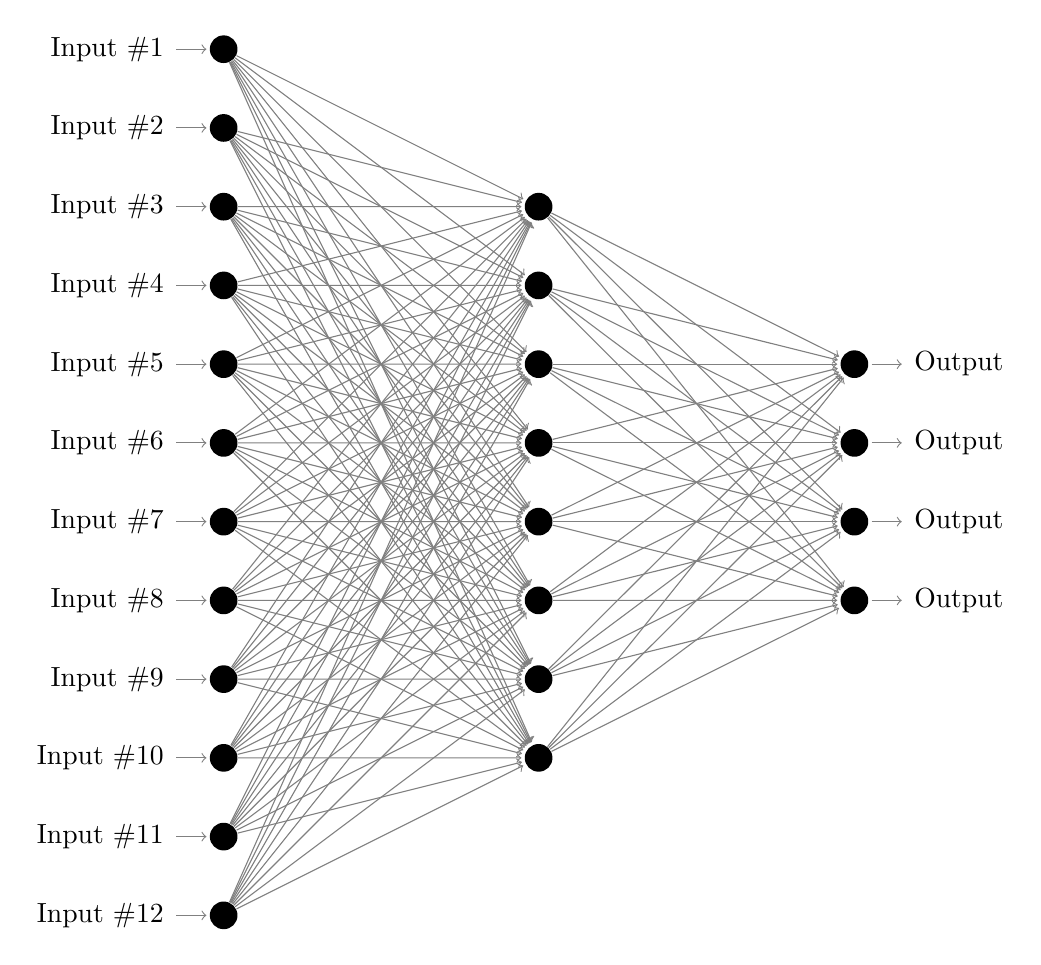
\begin{tikzpicture}[shorten >=1pt,->,draw=black!50, node distance=.3\layersep]
      \tikzstyle{every pin edge}=[<-,shorten <=1pt]
      \tikzstyle{neuron}=[circle,fill=black,minimum size=10pt,inner sep=0pt]
      \tikzstyle{input neuron}=[neuron];
      \tikzstyle{output neuron}=[neuron];
      \tikzstyle{hidden neuron}=[neuron];
      \tikzstyle{annot} = [text width=2em, text centered]

      % Draw the input layer nodes
      \foreach \name / \y in {1,...,12}
      % This is the same as writing \foreach \name / \y in {1/1,2/2,3/3,4/4}
          \node[input neuron, pin=left:Input \#\y] (I-\name) at (0,-\y) {};

      % Draw the hidden layer nodes
      \foreach \name / \y in {1,...,8}
          \path[yshift=-2cm]
              node[hidden neuron] (H-\name) at (4\layersep,-\y cm) {};

      % Draw the hidden layer nodes
      \foreach \name / \y in {1,...,4}
          \path[yshift=-4cm]
              node[output neuron, pin={[pin edge={->}]right:Output}, right of=H-3] (O-\name) at (8\layersep,-\y cm) {};


      % Connect every node in the input layer with every node in the
      % hidden layer.
      \foreach \source in {1,...,12}
          \foreach \dest in {1,...,8}
              \path (I-\source) edge (H-\dest);

      % Connect every node in the hidden layer with the output layer
      \foreach \source in {1,...,8}
          \foreach \dest in {1,...,4}
              \path (H-\source) edge (O-\dest);
  \end{tikzpicture}

  \caption{FFNN snake controller}
  \label{ffnn_snake}
\end{figure}

\paragraph{Fitness Function and Evaluation}

The objective function, which is run by the optimization algorithms, takes the evolved weights of the neural network and attempts to play the game using them. The fitness function of gameplay if determined by the equation~\ref{eq:snake_fitness}.

\begin{equation} \label{eq:snake_fitness}
  fitness = \text{foodEaten} + \frac{1}{1-e^{-\text{movesMade}}}
\end{equation}

The fitness function ensured that the snake has an ``easy start'' when it will be rewarded for not dying, but then has to pursue food in order to maximize it's fitness.


\subsection{Results}

This section presents results for the benchmarks of the four algorithms presented in this thesis.

\paragraph{Function Optimization at D=10}
DEDA significantly outperforms the other algorithms at most unimodal functions. DE significantly outperforms the others at one unimodal and one multimodal function. PSO outperforms the others by a slight margin on most multimodal function. Separability does not seem to influence the results. Table~\ref{table:f_res_10} presents the data.

For $F_1$ EDA significantly outperforms DE and PSO, while DEDA lags far behind. For $F_2$ DEDA finds significantly better results than the rests, while EDA performs the worst. For $F_3$ DEDA performs best followed by DE, but PSO and EDA do not find good solutions at all. For $F_4$ DEDA significantly outperforms the rest and EDA does not find any good results at all. For $F_5$ DE significantly outperforms the rest, DEDA finds an acceptable results and PSO and EDA do not find any good results. For $F_6$ DE significantly outperforms the rest, DEDA finds an acceptable results and PSO and EDA do not find any good results. For $F_7$ EDA find the best solution but all algorithms achieve similar results. For $F_8$ PSO find the best solution but all algorithms achieve similar results. For $F_9$ PSO find the best solution but all algorithms achieve similar results. For $F_{10}$ PSO find the best solution but all algorithms achieve similar results.

\begin{table}[H]
  \centering
  \begin{center}
    \footnotesize
    \begin{tabular}{ | c | c | c | c | c | c | c | c | c | }
      \hline
      F & \multicolumn{2}{c|}{DE} & \multicolumn{2}{c|}{PSO} & \multicolumn{2}{c|}{EDA} & \multicolumn{2}{c |}{DEDA} \\ \hline
      & Avg & Std & Avg & Std & Avg & Std & Avg & Std \\ \hline
      1 & 3,88E-17 & 3,42E-17 & 1,65E-16 & 3,64E-16 & \textbf{1,67E-27} & 4,07E-28 & 0,00E+00 & 0,00E+00 \\ \hline
      2 & 1,83E-08 & 1,24E-08 & 2,07E-06 & 3,36E-06 & 2,51E+02 & 1,42E+02 & \textbf{4,23E-27} & 3,10E-27 \\ \hline
      3 & 5,19E-01 & 2,29E-01 & 4,88E+05 & 7,21E+05 & 1,09E+05 & 8,32E+04 & \textbf{4,96E-02} & 3,01E-02 \\ \hline
      4 & 3,36E-07 & 2,59E-07 & 6,31E-05 & 9,10E-05 & 3,21E+02 & 2,16E+02 & \textbf{1,73E-26} & 2,16E-26 \\ \hline
      5 & \textbf{4,24E-13} & 7,82E-13 & 4,94E+02 & 4,49E+02 & 1,67E+02 & 1,37E+02 & 6,57E+00 & 1,26E+01 \\ \hline
      6 & \textbf{5,43E-05} & 1,24E-04 & 2,11E+02 & 7,15E+02 & 1,34E+04 & 4,30E+04 & 6,71E+00 & 5,83E-01 \\ \hline
      7 & 4,87E-01 & 7,61E-02 & 2,74E-01 & 1,79E-01 & \textbf{1,87E-01} & 2,23E-01 & 3,41E-01 & 1,24E-01 \\ \hline
      8 & 2,04E+01 & 7,20E-02 & \textbf{2,03E+01} & 8,82E-02 & 2,04E+01 & 8,15E-02 & 2,04E+01 & 6,88E-02 \\ \hline
      9 & 2,50E+01 & 4,44E+00 & \textbf{1,76E+00} & 1,49E+00 & 2,35E+01 & 3,08E+00 & 1,80E+01 & 3,52E+00 \\ \hline
      10 & 3,26E+01 & 4,25E+00 & \textbf{1,73E+01} & 7,50E+00 & 2,11E+01 & 3,43E+00 & 2,05E+01 & 3,62E+00 \\ \hline
    \end{tabular}
  \end{center}
  \caption{Benchmark results for $F_{1-10}$ $D=10$}
  \label{table:f_res_10}
\end{table}

\paragraph{Function Optimization at D=30}
DEDA moderately outperform the other algorithms at most unimodal functions. PSO outperform all other algorithms on the multimodal functions, but the results are fairly even. DEDA significantly outperforms the others on separable unimodal algorithms. Table~\ref{table:f_res_30} presents the data.

For $F_1$ DEDA performs best closely followed by EDA. PSO also finds a good result but DE finds a significantly worse result. For $F_2$ all algorithms find similar solutions and DEDA finds the best one. For $F_3$ all algorithms find similar solutions and EDA finds the best one. For $F_4$ all algorithms find somewhat similar solutions and DEDA finds the best one. For $F_5$ all algorithms find somewhat similar solutions and DEDA finds the best one. For $F_6$ all algorithms find somewhat similar solutions and DEDA finds the best one. For $F_7$ PSO finds the best solution followed EDA and DE and  DEDA find worse solutions. For $F_8$ all algorithms find similar solutions and PSO finds the best one. For $F_9$ DE, EDA and DEDA find similar solutions, but PSO finds a somewhat better solution. For $F_{10}$ all algorithms find similar solutions and PSO finds the best one.

\begin{table}[H]
  \centering
  \begin{center}
    \footnotesize
    \begin{tabular}{ | c | c | c | c | c | c | c | c | c | }
      \hline
      F & \multicolumn{2}{c|}{DE} & \multicolumn{2}{c|}{PSO} & \multicolumn{2}{c|}{EDA} & \multicolumn{2}{c |}{DEDA} \\ \hline
      & Avg & Std & Avg & Std & Avg & Std & Avg & Std \\ \hline
      1 & 1,03E+00 & 1,53E-01 & 4,54E-10 & 7,66E-10 & 1,81E-25 & 7,66E-10 & \textbf{8,58E-28} & 1,40E-28 \\ \hline
      2 & 3,07E+03 & 6,91E+02 & 1,42E+03 & 7,01E+02 & 1,71E+03 & 7,01E+02 & \textbf{4,84E+02} & 1,80E+02 \\ \hline
      3 & 3,28E+07 & 5,84E+06 & 1,92E+07 & 1,12E+07 & \textbf{4,93E+06} & 1,12E+07 & 1,88E+07 & 4,86E+06 \\ \hline
      4 & 6,06E+03 & 1,23E+03 & 1,50E+04 & 6,87E+03 & 3,63E+03 & 6,87E+03 & \textbf{6,74E+02} & 1,96E+02 \\ \hline
      5 & 1,38E+03 & 3,54E+02 & 6,92E+03 & 2,55E+03 & 2,70E+03 & 2,55E+03 & \textbf{1,31E+02} & 9,21E+01 \\ \hline
      6 & 2,99E+03 & 1,24E+03 & \textbf{5,30E+02} & 8,60E+02 & 8,57E+04 & 8,60E+02 & 7,32E+03 & 2,21E+04 \\ \hline
      7 & 1,22E+00 & 5,36E-02 & \textbf{5,77E-02} & 5,18E-02 & 5,86E+00 & 5,18E-02 & 2,54E-01 & 4,25E-01 \\ \hline
      8 & 2,09E+01 & 4,24E-02 & \textbf{2,09E+01} & 5,74E-02 & 2,10E+01 & 5,74E-02 & 2,10E+01 & 5,41E-02 \\ \hline
      9 & 1,91E+02 & 9,58E+00 & \textbf{2,53E+01} & 5,97E+00 & 1,53E+02 & 5,97E+00 & 1,60E+02 & 8,27E+00 \\ \hline
      10 & 2,19E+02 & 1,09E+01 & \textbf{1,14E+02} & 3,78E+01 & 1,59E+02 & 3,78E+01 & 1,60E+02 & 8,53E+00 \\ \hline
    \end{tabular}
  \end{center}
  \caption{Benchmark results for $F_{1-10}$ $D=30$}
  \label{table:f_res_30}
\end{table}

\paragraph{Function Optimization at D=50}
The results are fairly even. DEDA significantly outperforms the others on separable unimodal algorithms. The multimodal functions favor PSO, the unimodal function favor UMDA while DEDA's results are more scattered. Table~\ref{table:f_res_50} presents the data.

For $F_1$ DEDA find the best results closely followed by EDA. DE finds a bad solution and PSO is in-between DE and EDA.
For $F_2$ DE, PSO and DEDA find similar solutions. EDA outperforms the all by a moderate margin.
For $F_3$ all algorithms perform similarly. EDA performs best, followed by PSO.
For $F_4$ EDA performs best, followed by DE and DEDA. PSO finds the worst solution.
For $F_5$ DEDA finds the best solution, closely followed by EDA, while DE and PSO find somewhat worse solutions.
For $F_6$ DE performs signigicantly worse than the rest, which perform very similarly. EDA finds the best solution.
For $F_7$ DEDA finds a good solution while PSO performs somewhat poorer and DE and EDA find the worst solutions.
For $F_8$ all algorithms find similar solutions. PSO finds the best solution.
For $F_9$ all algorithms find somewhat similar solutions. PSO finds the best solution.
For $F_{10}$ all algorithms find similar solutions. PSO finds the best solution.

\begin{table}[H]
  \centering
  \begin{center}
    \footnotesize
    \begin{tabular}{ | c | c | c | c | c | c | c | c | c | }
      \hline
      F & \multicolumn{2}{c|}{DE} & \multicolumn{2}{c|}{PSO} & \multicolumn{2}{c|}{EDA} & \multicolumn{2}{c |}{DEDA} \\ \hline
      & Avg & Std & Avg & Std & Avg & Std & Avg & Std \\ \hline
      1 & 5,64E+02 & 8,54E+01 & 1,20E-04 & 1,49E-04 & 1,04E-24 & 9,53E-26 & \textbf{2,14E-26} & 4,42E-27 \\ \hline
      2 & 5,00E+04 & 4,88E+03 & 3,69E+04 & 1,02E+04 & \textbf{3,55E+03} & 6,45E+02 & 3,96E+04 & 5,00E+03 \\ \hline
      3 & 2,52E+08 & 3,33E+07 & 8,68E+07 & 4,64E+07 & \textbf{1,31E+07} & 2,94E+06 & 1,96E+08 & 3,16E+07 \\ \hline
      4 & 7,02E+04 & 9,89E+03 & 1,12E+05 & 3,09E+04 & \textbf{8,17E+03} & 1,71E+03 & 5,08E+04 & 7,70E+03 \\ \hline
      5 & 1,33E+04 & 1,03E+03 & 1,48E+04 & 3,64E+03 & 4,31E+03 & 2,95E+02 & \textbf{2,71E+03} & 3,84E+02 \\ \hline
      6 & 7,19E+06 & 2,18E+06 & 1,62E+04 & 3,11E+04 & \textbf{1,18E+04} & 2,68E+04 & 2,23E+04 & 1,09E+05 \\ \hline
      7 & 3,32E+01 & 6,43E+00 & 1,05E+00 & 1,24E-01 & 1,25E+01 & 3,91E+00 & \textbf{6,04E-01} & 6,19E-01 \\ \hline
      8 & 2,12E+01 & 2,28E-02 & \textbf{2,11E+01} & 5,09E-02 & 2,11E+01 & 4,97E-02 & 2,11E+01 & 3,28E-02 \\ \hline
      9 & 3,94E+02 & 1,24E+01 & \textbf{7,93E+01} & 1,46E+01 & 3,14E+02 & 1,41E+01 & 3,27E+02 & 1,13E+01 \\ \hline
      10 & 4,48E+02 & 1,87E+01 & \textbf{2,79E+02} & 6,36E+01 & 3,20E+02 & 1,17E+01 & 3,27E+02 & 9,26E+00 \\ \hline
    \end{tabular}
  \end{center}
  \caption{Benchmark results for $F_{1-10}$ $D=50$}
  \label{table:f_res_50}
\end{table}

\paragraph{Function Approximation}
The results are fairly even but DEDA performs best overall. PSO is second best. Table~\ref{table:fa_res} presents the data.

For $simplefit$ DE and PSO find the best solutions. For $bodyfat$ DEDA finds the best solution but all algorithms deliver similar results. For $chemical$ DEDA, PSO and DE find similar solutions. DEDA performs best and EDA finds a much worse solution. For $cho$ PSO finds the best solution but all algorithms deliver similar results. For $engine$ DEDA performs best, closelly followed by PSO. DE and EDA perform somewhat worse. For $house$ PSO finds the best solution but all algorithms deliver similar results.

\begin{table}[H]
  \centering
  \begin{center}
    \scriptsize
    \begin{tabular}{ | c | c | c | c | c | c | c | c | c | }
      \hline
      F & \multicolumn{2}{c|}{DE} & \multicolumn{2}{c|}{PSO} & \multicolumn{2}{c|}{EDA} & \multicolumn{2}{c |}{DEDA} \\ \hline
       & Avg & Std & Avg & Std & Avg & Std & Avg & Std \\ \hline
       simplefit	&	\textbf{6,91E-01}	&	1,67E-16	&	6,91E-01	&	3,90E-04	&	6,64E+00	&	7,12E-01	&	1,09E+00	&	1,13E-01 \\ \hline
       bodyfat	&	1,92E+01	&	2,59E+00	&	1,90E+01	&	2,14E+00	&	1,96E+01	&	2,11E+00	&	\textbf{1,69E+01}	&	1,26E+00 \\ \hline
       chemical	&	2,58E+01	&	5,53E-04	&	2,46E+01	&	1,97E+00	&	1,15E+05	&	2,38E+03	&	\textbf{2,43E+01}	&	2,11E+00 \\ \hline
       cho	&	2,07E+03	&	2,16E+02	&	\textbf{1,86E+03}	&	4,84E+01	&	5,32E+03	&	6,24E+02	&	1,97E+03	&	1,10E+02 \\ \hline
       engine	&	1,29E+05	&	7,09E+04	&	7,86E+04	&	6,86E+03	&	9,91E+05	&	2,59E+03	&	\textbf{5,61E+04}	&	1,27E+04 \\ \hline
       house	&	3,19E+01	&	4,81E-01	&	\textbf{2,00E+01}	&	1,93E+00	&	2,45E+01	&	2,68E+00	&	2,03E+01	&	5,90E+00 \\ \hline
    \end{tabular}
  \end{center}
  \caption{Benchmark results for $F_{1-10}$}
  \label{table:fa_res}
\end{table}

\paragraph{Classification}
DEDA and UMDA perform best. The results are even overall. Table~\ref{table:cls_res} presents the data.

For $simpleclass$ DEDA finds the best solution but all algorithms deliver similar results. All algorithms find good solution for $cancer$ but EDA has a slight edge. For $crab$ EDA finds the best solutions, closely followed by PSO and DE, while DEDA finds a somewhat worse solution. For $glass$ PSO finds the best solutions, closely followed by EDA and DEDA, while DE finds a somewhat worse solution. For $iris$ DEDA finds the best solution and DE, PSO and EDA find somewhat worse solutions. For $thyroid$ EDA finds the best solution but all algorithms deliver similar results. For $wine$ DEDA finds the best solution but all algorithms deliver similar results.

\begin{table}[H]
  \centering
  \begin{center}
    \footnotesize
    \begin{tabular}{ | c | c | c | c | c | c | c | c | c | }
      \hline
      F & \multicolumn{2}{c|}{DE} & \multicolumn{2}{c|}{PSO} & \multicolumn{2}{c|}{EDA} & \multicolumn{2}{c |}{DEDA} \\ \hline
       & Avg & Std & Avg & Std & Avg & Std & Avg & Std \\ \hline
       simpleclass & 1,76E-01	&	1,29E-02	&	1,83E-01	&	7,07E-03	&	1,97E-01	&	2,56E-02	&	\textbf{1,43E-01}	&	7,76E-03 \\ \hline
       cancer  & 7,74E-02	&	9,95E-03	&	6,48E-02	&	1,40E-02	&	\textbf{3,23E-02}	&	9,32E-04	&	5,26E-02	&	6,65E-03 \\ \hline
       crab  & 1,83E-01	&	3,25E-02	&	1,27E-01	&	2,54E-02	&	\textbf{1,20E-01}	&	3,70E-02	&	6,35E-02	&	5,26E-02 \\ \hline
       glass &  1,25E-01	&	3,54E-02	&	\textbf{7,45E-02}	&	1,95E-02	&	9,71E-02	&	2,11E-02	&	9,91E-02	&	4,33E-02 \\ \hline
       iris  & 1,63E-01	&	7,31E-03	&	1,26E-01	&	3,22E-02	&	1,31E-01	&	3,18E-02	&	\textbf{6,67E-02}	&	5,23E-02 \\ \hline
       thyroid &  2,00E-01	&	3,66E-02	&	2,25E-01	&	4,84E-02	&	\textbf{1,17E-01}	&	1,24E-02	&	1,80E-01	&	3,57E-02 \\ \hline
       wine  & 3,45E-01	&	2,33E-02	&	3,06E-01	&	2,25E-02	&	2,79E-01	&	2,52E-02	&	\textbf{2,59E-01}	&	7,80E-02 \\ \hline
    \end{tabular}
  \end{center}
  \caption{Benchmark results for $CLS_{1-6}$}
  \label{table:cls_res}
\end{table}

\paragraph{Clustering}
The results are fairly even but DEDA performs best overall. Table~\ref{table:clu_res} presents the data.

\begin{table}[H]
  \centering
  \begin{center}
    \footnotesize
    \begin{tabular}{ | c | c | c | c | c | c | c | c | c | }
      \hline
      F & \multicolumn{2}{c|}{DE} & \multicolumn{2}{c|}{PSO} & \multicolumn{2}{c|}{EDA} & \multicolumn{2}{c |}{DEDA} \\ \hline
       & Avg & Std & Avg & Std & Avg & Std & Avg & Std \\ \hline
      simplecluster	&	1,65E-01	&	1,39E-02	&	1,74E-01	&	1,57E-02	&	2,17E-01	&	2,05E-02	&	\textbf{1,51E-01}	&	8,12E-03 \\ \hline
    \end{tabular}
  \end{center}
  \caption{Benchmark results for $CLU_{1}$}
  \label{table:clu_res}
\end{table}

\paragraph{Intelligent Game Controllers}
DE performs significantly worse than the other algorithms. PSO, UMDA and DEDA performs similarly, with PSO showing the best results. Table~\ref{table:snake_res} presents the data.


\begin{table}[H]
  \centering
  \begin{center}
    \footnotesize
    \begin{tabular}{ | c | c | c | c | c | c | c | c | c | }
      \hline
      F & \multicolumn{2}{c|}{DE} & \multicolumn{2}{c|}{PSO} & \multicolumn{2}{c|}{EDA} & \multicolumn{2}{c |}{DEDA} \\ \hline
       & Avg & Std & Avg & Std & Avg & Std & Avg & Std \\ \hline
      snake & 2,32E+01 & 2,19E+00 & \textbf{2,92E+01} & 4,16E+00 & 2,78E+01 & 1,34E+01 & 2,69E+01 & 3,59E+00 \\ \hline
    \end{tabular}
  \end{center}
  \caption{Benchmark results for $IGC_{1}$}
  \label{table:snake_res}
\end{table}


\subsection{Discussion}

PSO is the best algorithm for multimodal functions and also performs best at controlling neural networks in game controllers. DEDA performs well at unimodal function at all dimensions, while UMDA works well at higher dimensions. DEDA produces the best results when optimizing neural networks. UMDA also works well when optimizing neural networks for clustering.


\input{./results}

% ============================= Final words ============================

\input{./discussions}

\input{./conclusion}

\section{Future Work}

Since there exit many variations of the three popular algorithms presented in this thesis, it would be interesting to compare different varieties of algorithms which performed best on the machine learning problem sets in order to find specific optimization which work well with machine learning.



%\section{Acknowledgments}

Lorem ipsum dolor sit amet, consectetur adipiscing elit. Sed suscipit eu ante id aliquet. Class aptent taciti sociosqu ad litora torquent per conubia nostra, per inceptos himenaeos. Mauris condimentum iaculis erat, eget pretium leo consequat eget. Donec eu aliquam purus. Quisque scelerisque feugiat ligula, non vehicula urna blandit nec. Etiam a dignissim purus, at molestie dui. Vestibulum a venenatis mi, id hendrerit sem. Cras purus elit, dapibus eget est id, lacinia tincidunt neque. Mauris eu arcu ipsum. Sed enim leo, iaculis vitae nisl tincidunt, ultricies accumsan diam. Donec neque urna, pellentesque sit amet interdum a, pretium ac enim. Proin quis ante nunc. Fusce vitae lorem condimentum, porta velit blandit, commodo nisi.


% ============================= References ============================
\newpage
%\textbf{Referenser (References)}

F\"or examensarbeten ska du ha vetenskapliga referenser. En vetenskaplig referens \"ar en referens till en artikel som publicerats med syfte att sprida kunskap som resultat av metodiskt rigor\"ost driven forskning kring en forskningsfr\r{a}ga. Artikeln har granskats kollegialt genom s.k peer review och publicerats i en tidskrift eller s.k. konferens-proceedings. En vetenskaplig referens har grundl\"aggande information f\"or att identifiera artikeln: f\"orfattare, \r{a}rtal, titel, namn p\r{a} konferens eller tidskrift med volym, nummer och sidor samt f\"orlag. F\"or vetenskapliga referenser ska du inte ange DOI, URL eller n\"ar du h\"amtade den. Alla andra referenser har ett mindre vetenskapligt v\"arde: l\"arob\"ocker, studentuppsatser, journalistiska tidskrifter, branschtidskrifter, standards, popul\"arvetenskapliga publikationer, wikipedia, uppslagsverk, web-l\"ankar, TV- och radioprogram, bloggar och inl\"agg, alla dessa \"ar s\r{a}ledes inte vetenskapliga referenser. De kan anv\"andas som referenser men betraktas som komplement till de vetenskapliga referenserna.

Referenser ska anges enligt IEEE-standarden. I den l\"opande texten anger du referenserna med siffror (l\"opnummer) i hakparentes, t ex [1] i den ordning de f\"orekommer f\"orsta g\r{a}ngen i texten. F\"orekommer en referens flera g\r{a}nger i texten ska den anges med samma nummer varje g\r{a}ng. Om du vill ange ett kapitel eller en eller flera specifika sidor i referensen s\r{a} skriver du det efter l\"opnumret inom hakparentesen. T ex om du har ett citat ur en text s\r{a} anges detta med sidnummer, ex [2 s. 3]
N\"ar du s\"atter ut referenser i texten, s\r{a} t\"ank p\r{a} att de ska placeras i n\"ara anslutning till det som referensen handlar om, och alltid inom en mening, dvs f\"ore ’.’ Undantag fr\r{a}n detta \"ar om ett helt stycke behandlar samma referens, d\r{a} kan referensen s\"attas efter styckets slut.

Sist i rapporten ska det finnas en referenslista. I den ska finnas samtliga referenser du \r{a}beropar i texten, och du m\r{a}ste ocks\r{a} se till att du i texten verkligen refererar till samtliga i listan. L\"as om hur du anger k\"allorna i referenslistan p\r{a} \url{http://www.ieee.org/documents/ieeecitationref.pdf} alternativt i manualen \url{https://www.ieee.org/documents/style_manual.pdf}. Du kan ocks\r{a} g\r{a} via bibliotekets lista \"over guider till olika referensstilar som du hittar p\r{a} \url{http://www.mdh.se/bibliotek/kurser-stod/referera/guider-till-olika-referensstilar-1.79882?l=sv_SE}

Det \"ar mycket viktigt att referenshanteringen \"ar korrekt, b\r{a}de inne i texten och i sj\"alva listan! Detta \"ar en sak vi alltid tittar p\r{a} n\"ar vi bed\"omer rapporten. 

Det finns ocks\r{a} verktyg som hj\"alper dig att hantera referenser r\"att, Endnote (f\"or Word), se \url{http://www.mdh.se/bibliotek/kurser-stod/referera/endnote/} eller BibTex (f\"or LaTeX), se \url{http://www.bibtex.org/}.






\bibliographystyle{IEEEtran}
\bibliography{./references}
\addcontentsline{toc}{section}{References}

% ============================ Appendices =============================
\newpage
%\begin{appendices}

	%\section{Algorithms}

This appendix will present the matlab code for the four algorithms descibed under ``Algorithms''.

\subsection{Differential Evolution}

\inputminted{C}{DE.m}

	%\clearpage

	%\input{./Appendices/appendices2}
	%\clearpage

%\end{appendices}

\end{document}
